\documentclass[tikz, border=10pt]{standalone}
\usetikzlibrary{arrows.meta}
\begin{document}
    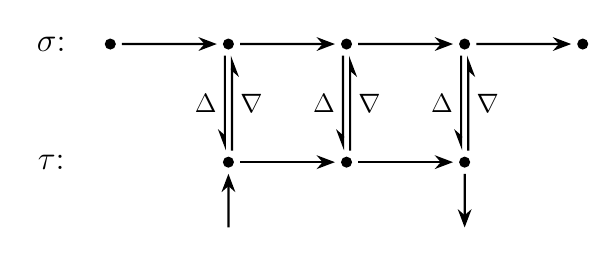
\begin{tikzpicture}[
        scale=1.5,
        point/.style={circle, fill=black, minimum size=4pt, inner sep=0pt},
        shortstyle/.style={thick, shorten >=2pt,shorten <=2pt},
        arrow/.style={-Stealth, shortstyle},
        foo/.tip={Stealth[harpoon,swap]},
        every node/.style={font=\large}
        ]
        \node at (-0.5,1) {$\sigma$:};
        \foreach \i in {0,...,4} {
            \node[point] (s\i) at (\i,1) {};
        }
        \foreach \i in {0,...,3} {
            \draw[arrow] (s\i) -- (s\the\numexpr\i+1);
        }
        \node at (-0.5,0) {$\tau$:};
        \foreach \i in {1,...,3} {
            \node[point] (t\i) at (\i,0) {};
        }
        \foreach \i in {1,2} {
            \draw[arrow] (t\i) -- (t\the\numexpr\i+1);
        }
        \foreach \i in {1,2,3} {
            \draw[shortstyle,-foo,transform canvas={xshift=-0.3ex}] (s\i) -- node[left,scale=.8] {$\Delta$} (t\i);
            \draw[shortstyle,foo-,transform canvas={xshift=+0.3ex}] (s\i) -- node[right,scale=.8] {$\nabla$} (t\i);
        }
        \draw[arrow] (1,-0.6) -- (t1);
        \draw[arrow] (t3) -- (3,-0.6);
    \end{tikzpicture}
\end{document}